\section{Introduction}

Microsoft Azure Storage is a global cloud storage system with a footprint in 38 geographic
regions~\cite{bib:azureregions}. Since 2010, Azure Storage has grown from tens of
petabytes to many exabytes, with tens of trillions of objects stored~\cite{greenberg15sdn}.

To protect customer data against disk, node, and rack failure within a data
center (DC), Azure Storage applies Local Reconstruction Coding (LRC)~\cite{huang12erasure}
to ensure high availability and durability. 
LRC significantly reduces the storage cost over the conventional scheme of
three-way replication.

To further protect customer data against catastrophic data center failures
(say due to earthquake, tsunami, etc.),
Azure Storage optionally replicate customer data to secondary DCs hundreds of miles away.
It is essential to the customers that even in the unlikely, albeit inevitable,
event of catastrophic data center failure, their data remain durable.

Geo-replication, however, doubles storage cost.
With many exabytes at present and exponential growth projected,
it is highly desirable to lower the storage cost
required for maintaining geo-redundancy.


%\begin{figure}[tp]
%\centering
%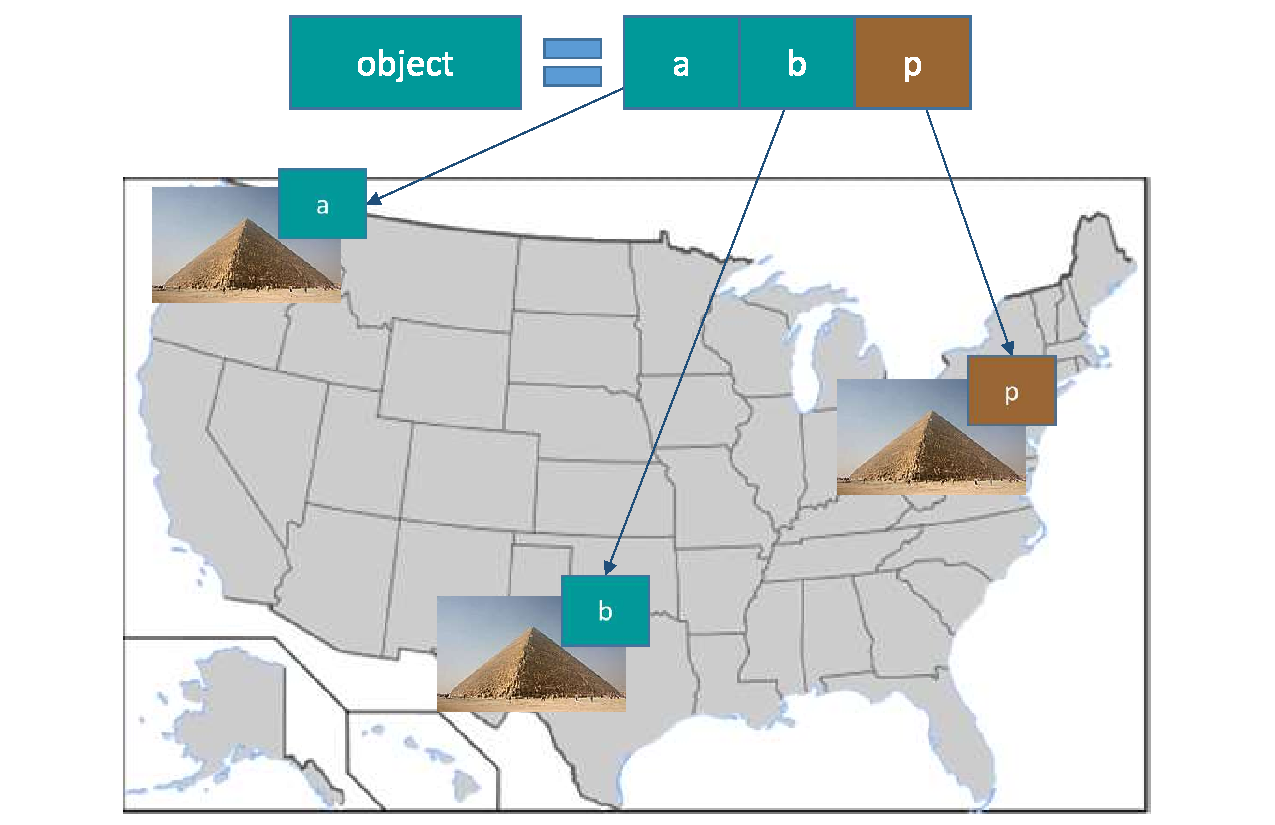
\includegraphics[width=0.4\textwidth]{images/giza_example_crop_fit}
%\caption{Storing Object in Giza}
%\label{fig:giza_example}
%\end{figure}

\begin{figure*}[!htbp]
\centering
%\hspace{-2em}
\begin{minipage}{0.3\textwidth}%
\centering
%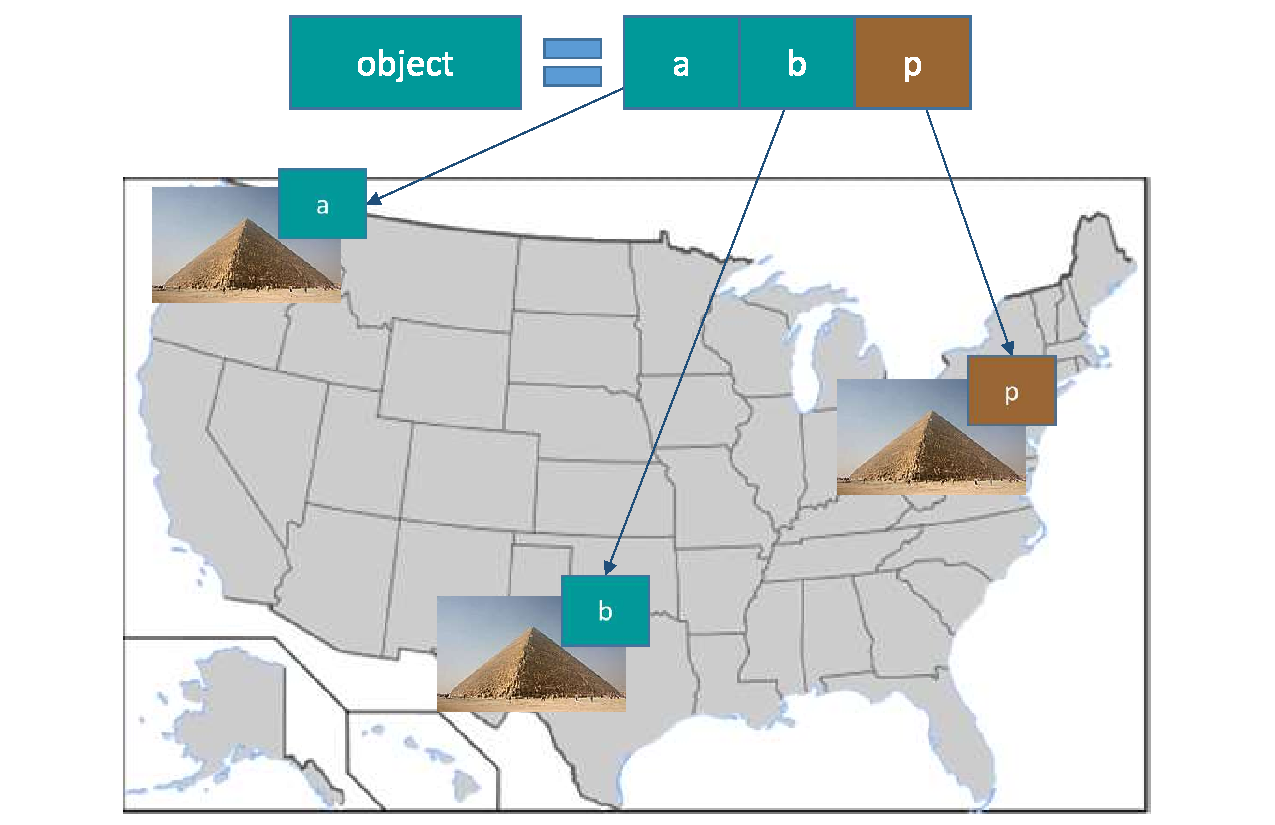
\includegraphics[width=\textwidth]{images/giza_example_crop_fit}
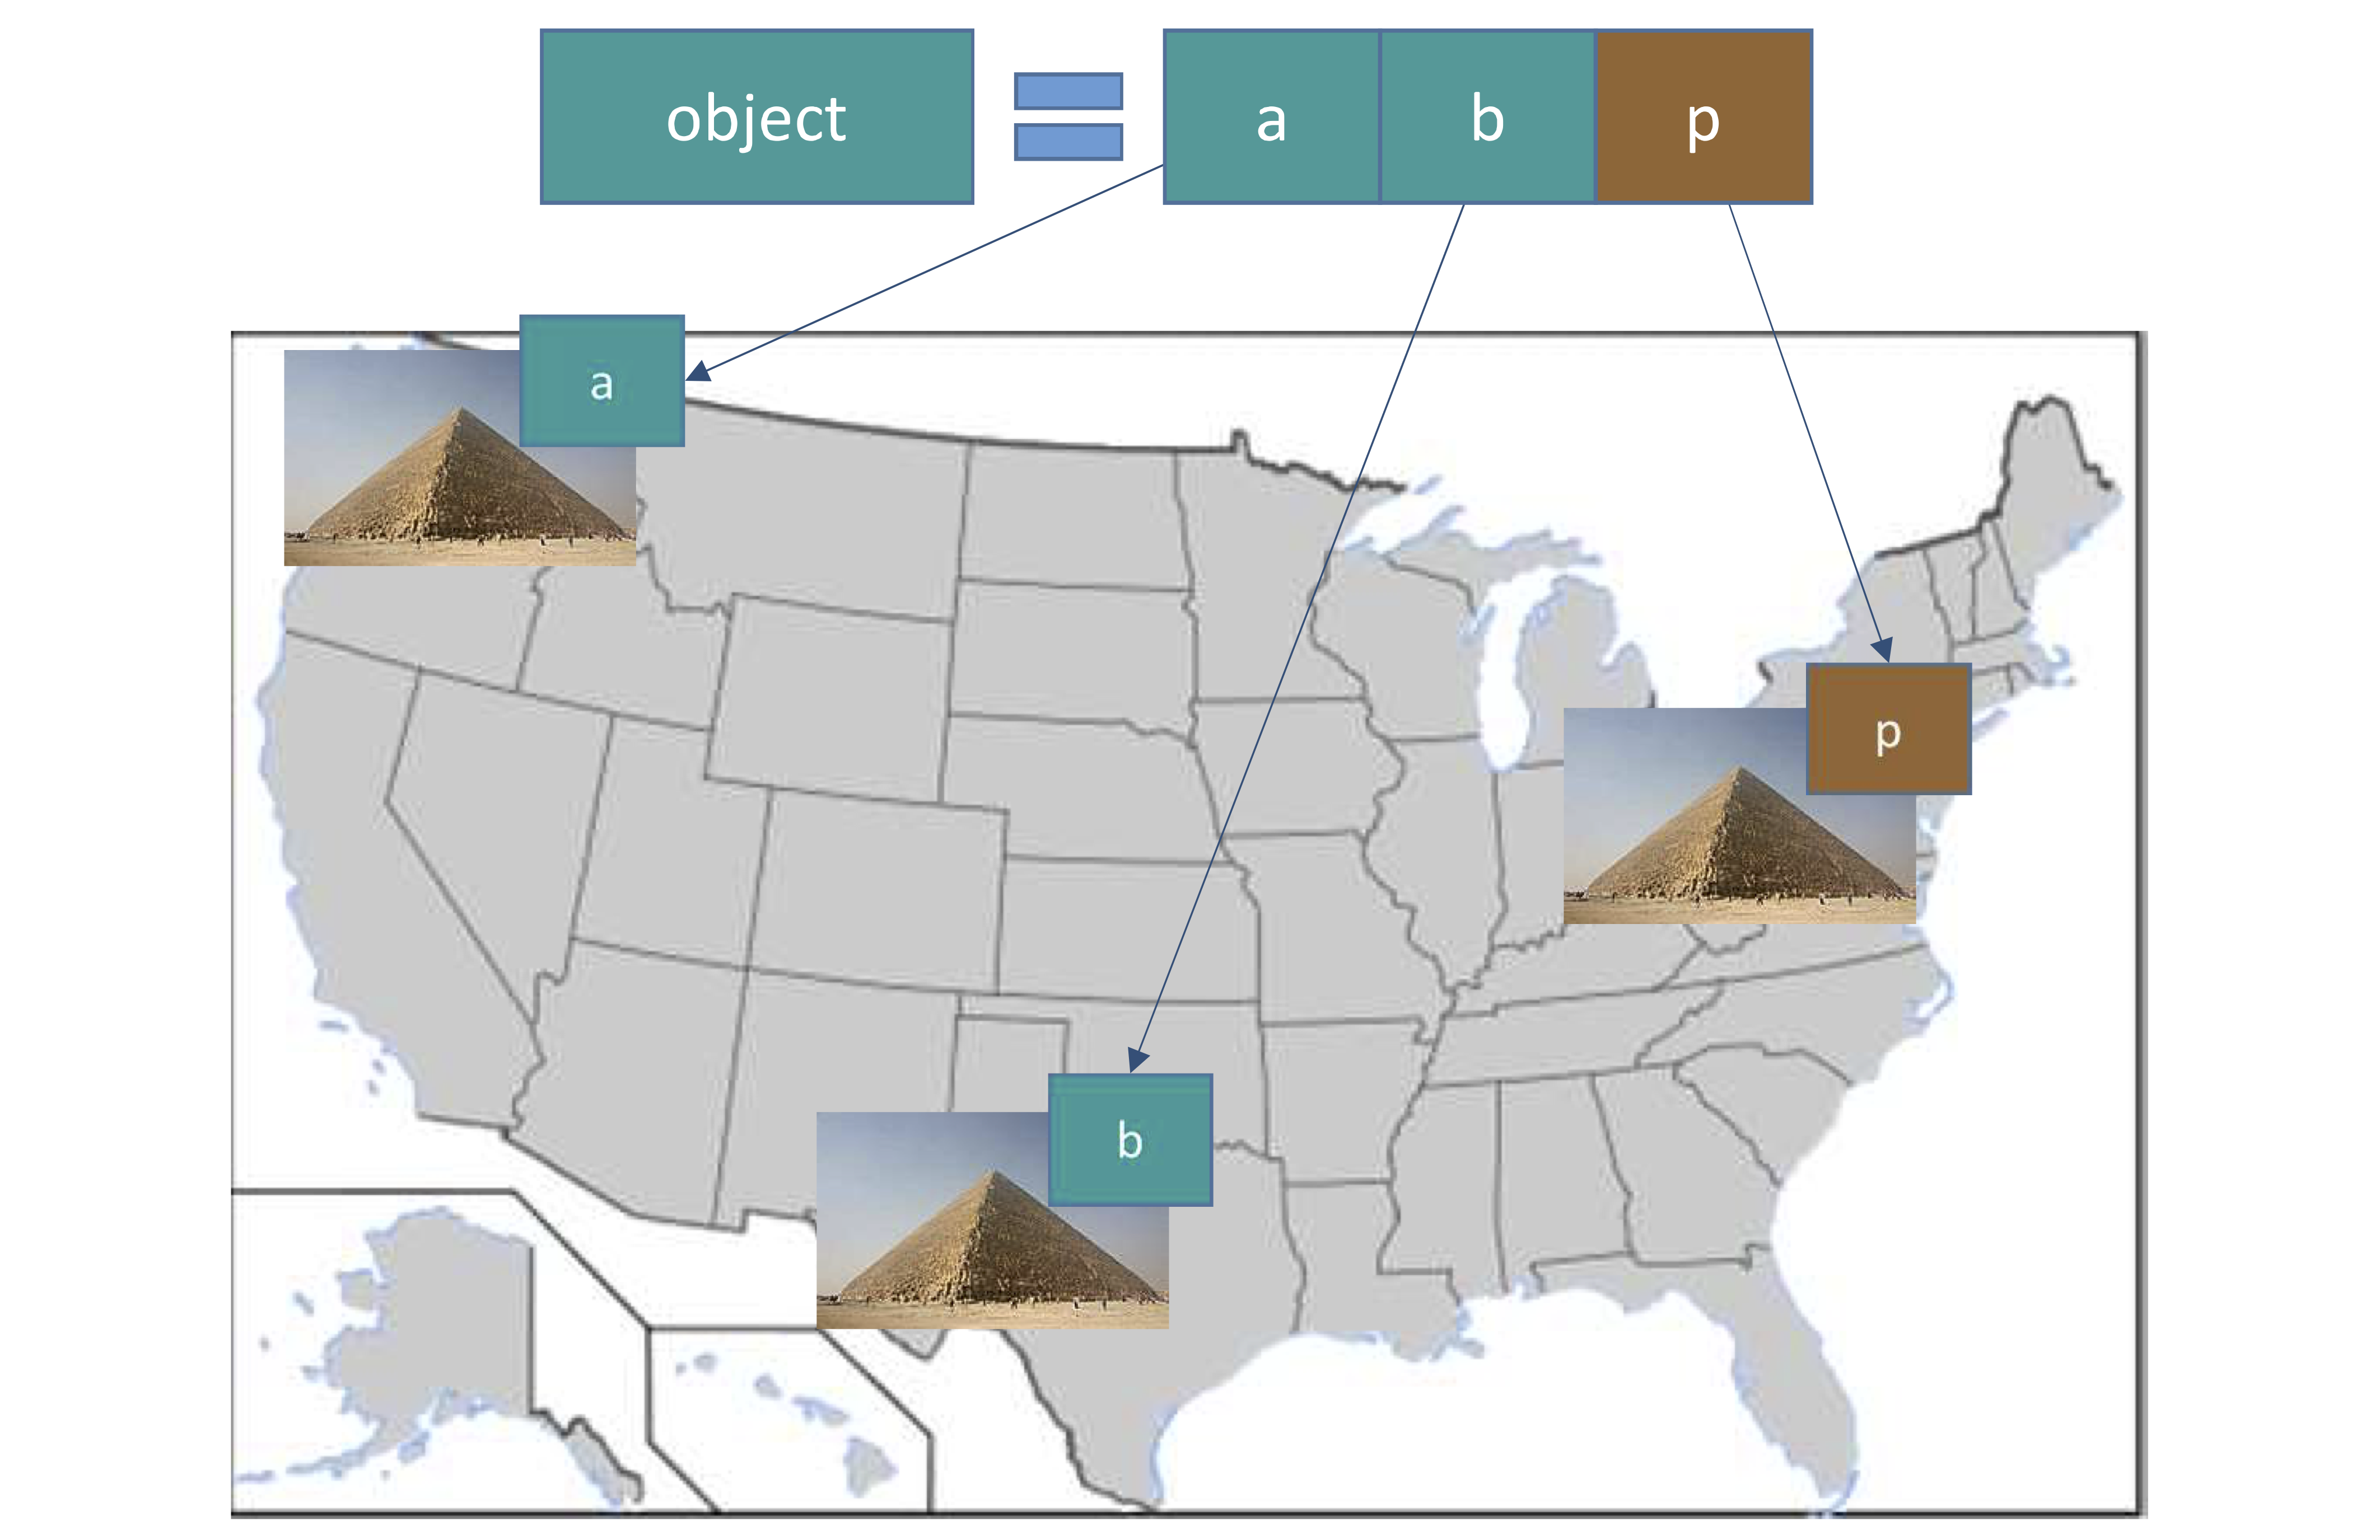
\includegraphics[width=\textwidth]{fig/giza_example_crop_fit}
\caption{Storing Object in Giza}
\label{fig:giza_example}
\end{minipage}%
\begin{minipage}{0.7\textwidth}%
\captionsetup{type=figure}
\centering
		\hspace{-1.5em}
    \subcaptionbox{\label{fig:object_size-storage_capacity}}
      {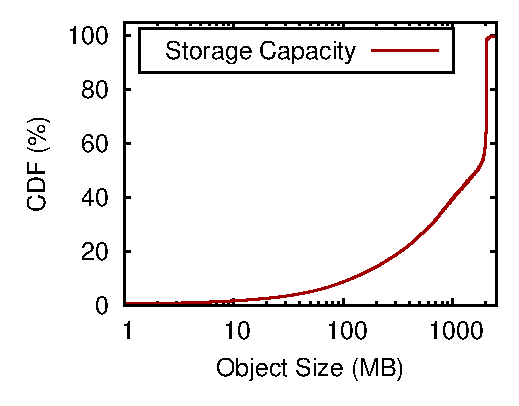
\includegraphics[height=0.275\textwidth]{data/object_size-storage_capacity}}%
		\hspace{-1em}
    \subcaptionbox{\label{fig:write_read_gap-bytes_read}}
      {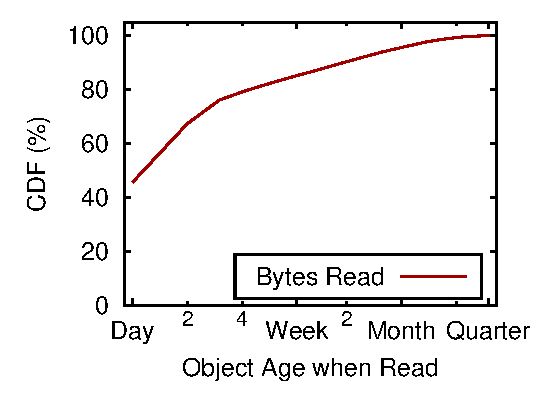
\includegraphics[height=0.275\textwidth]{data/write_read_gap-bytes_read}}%
		\hspace{-1.5em}
    \subcaptionbox{\label{fig:deletion}}
      {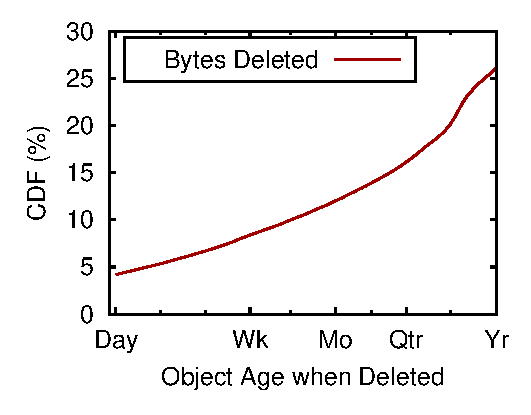
\includegraphics[height=0.275\textwidth]{data/age-bytes}}%
\caption{Microsoft OneDrive Characteristics}
\label{fig:case_for_giza}
%\end{figure}
\end{minipage}%

\end{figure*}
%%% Local Variables:
%%% mode: latex
%%% TeX-master: "main"
%%% End:


\subsection{Cross-DC Erasure Coding: Why Now?}

Erasure coding across geographically distributed DCs is an appealing option.
It has the potential to ensure durability in the face of data center failure
while significantly reducing storage cost compared to geo-replication.
The same economic argument that has driven cloud providers to erasure code data
within individual data centers naturally extends to the cross-DC scenario.

However, when customer data is erasure coded and striped across multiple DCs, 
serving read requests would require data retrieval from remote DCs, resulting in
cross-DC network traffic and latency. Furthermore, the recovery after catastrophic
DC failure would trigger wide-area erasure coding reconstruction. While such
reconstruction can be paced and prioritized based on demand, it nevertheless
requires sufficient cross-DC network bandwidth to ensure timely recovery.

Therefore, cross-DC erasure coding only becomes economically attractive if 1)
there are workloads that consume very large storage capacity while incurring very
little cross-DC traffic; 2) there are enough cross-DC network bandwidth at very
low cost.

For the former, Azure Storage indeed serves many customers
with such workloads. Using Microsoft OneDrive as an example,
Section~\ref{sec:motivation} illustrates the characteristics of typical cloud storage workloads
and why they are ideal for cross-DC erasure coding.
For the latter, recent technological breakthroughs~\cite{mears1986low, zhu2011112}
have dramatically increased bandwidth and reduced cost in cross-DC networking.
For example, Facebook and Microsoft have teamed up to build \textit{MAREA},
a new fiber optic cable under the Atlantic Ocean 
that will come online in 2017 with 160 Tbps capacity~\cite{bib:MAREA1, bib:MAREA2}.
The significant advancement in cross-DC networking is now making cross-DC erasure coding economically viable.

\comment{bib:MAREA1, http://www.wsj.com/articles/facebook-and-microsoft-to-build-fiber-optic-cable-across-atlantic-1464298853}
\comment{bib:MAREA2, http://www.usatoday.com/story/experience/2016/05/26/microsoft-facebook-undersea-cable-google-marea-amazon/84984882/}
\comment{bib:FA-1, https://en.wikipedia.org/wiki/Fiber-Optic_Link_Around_the_Globe}

\subsection{Challenges and Contributions}

Giza erasure codes and stripes customer data across multiple data centers,
so reads and writes require cross-DC communication. The latency is minimized when
reads and writes complete within single cross-DC round trip. This is not
difficult to achieve for typical Giza workloads, where objects are updated
infrequently.

Nevertheless, concurrent updates of same object do exist.
Giza needs to ensure strong consistency when conflicts occur. This becomes
particularly interesting as Giza allows requests to originate from any DC.
Consider two concurrent requests updating the same object (with different data)
from two separate data centers. Depending on network latency, the individual requests may
arrive at different data centers in different order. If not handled properly,
this would result in data inconsistency.

To ensure strong consistency, one possible approach is to dedicate a primary
data center that handles all updates and enforces execution order. This is less
than ideal because the requests from non-primary data centers have to be relayed
to the primary first. This would incur extra cross-DC latency, even when there are
no concurrent updates.


An ideal solution should optimize for the common case.
When there are no concurrent updates, 
reads and writes originating from any DC should complete within single cross-DC round trip.
In addition, the ideal solution should ensure strong consistency in the rare case,
when concurrent updates to the same object do sometimes occur.
It is expected and acceptable that latency would increase
as it takes multiple cross-DC round trips to resolve the conflicts.

Giza achieves the ideal solution and makes the following contributions:
\begin{itemize}
    \item We have designed and implemented Giza, a strongly consistent,
      versioned object store that erasure codes objects across globally
      distributed data centers.
    \item Giza achieves minimum latency in the common case and ensures strong consistency in the rare case.
    \item Giza applies well-known distributed algorithms -- Paxos~\cite{lamport01paxos}
      and Fast Paxos~\cite{lamport05fast} -- in a novel way on top of restricted cloud storage APIs.
    \item Giza is deployed in \deployment and experimental results demonstrate
      that it achieves our design goals.
\end{itemize}

%%% Local Variables:
%%% mode: latex
%%% TeX-master: "main"
%%% End: